Given our large scope, getting a good overview of our time and resources were crucial. From the get-go we set up some milestones and the deadlines. We modeled our whole project around meeting the milestones. We created a Gantt-diagram to visualize them.

In order to make sure we were progressing towards each milestone in a timely manner, we set up various meetings which often had small deadlines attached to them. Each meeting usually lasted 1 hour, and consisted of each member talking about their progress with their specific task and whom should be responsible for new tasks.

\begin{figure}[H]
	\centering
	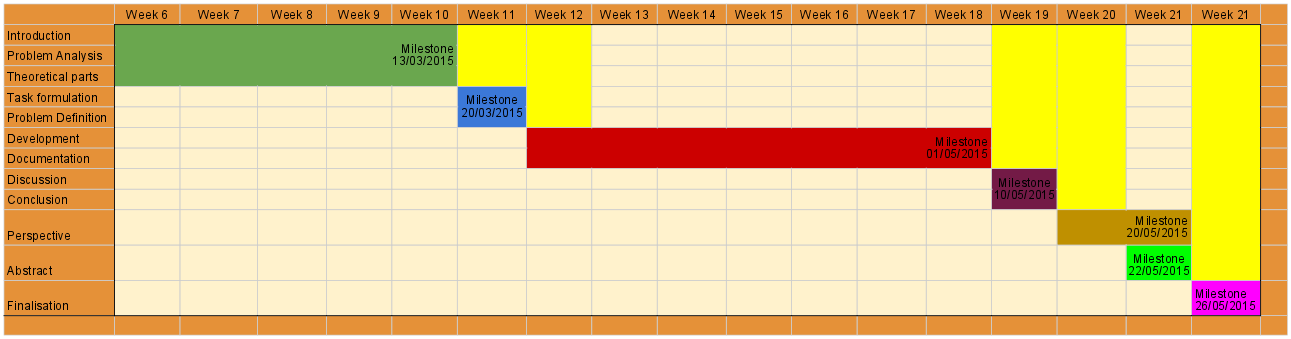
\includegraphics[scale=.35]{images/gantt1.png}
	\caption{Initial Gantt Diagram}
\end{figure}

As we were recieving the parts we ordered we realised they would not arrive in time for us to start development at the time we intended to. We then re-evaluated our milestones and came up with a revised Gantt-diagram.

\begin{figure}[H]
	\centering
	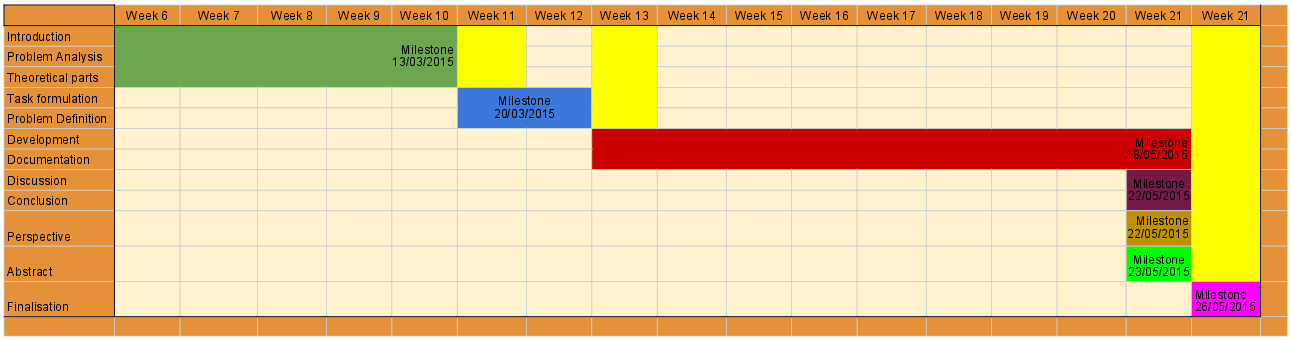
\includegraphics[scale=.35]{images/gantt2.png}
	\caption{Actual Gantt Diagram}
\end{figure}

We choose to use an online Kanban board for the purpose of keeping track of tasks. We separated tasks into 7 columns, each depicting a stage in the progress of the task.

\begin{figure}[H]
	\centering
	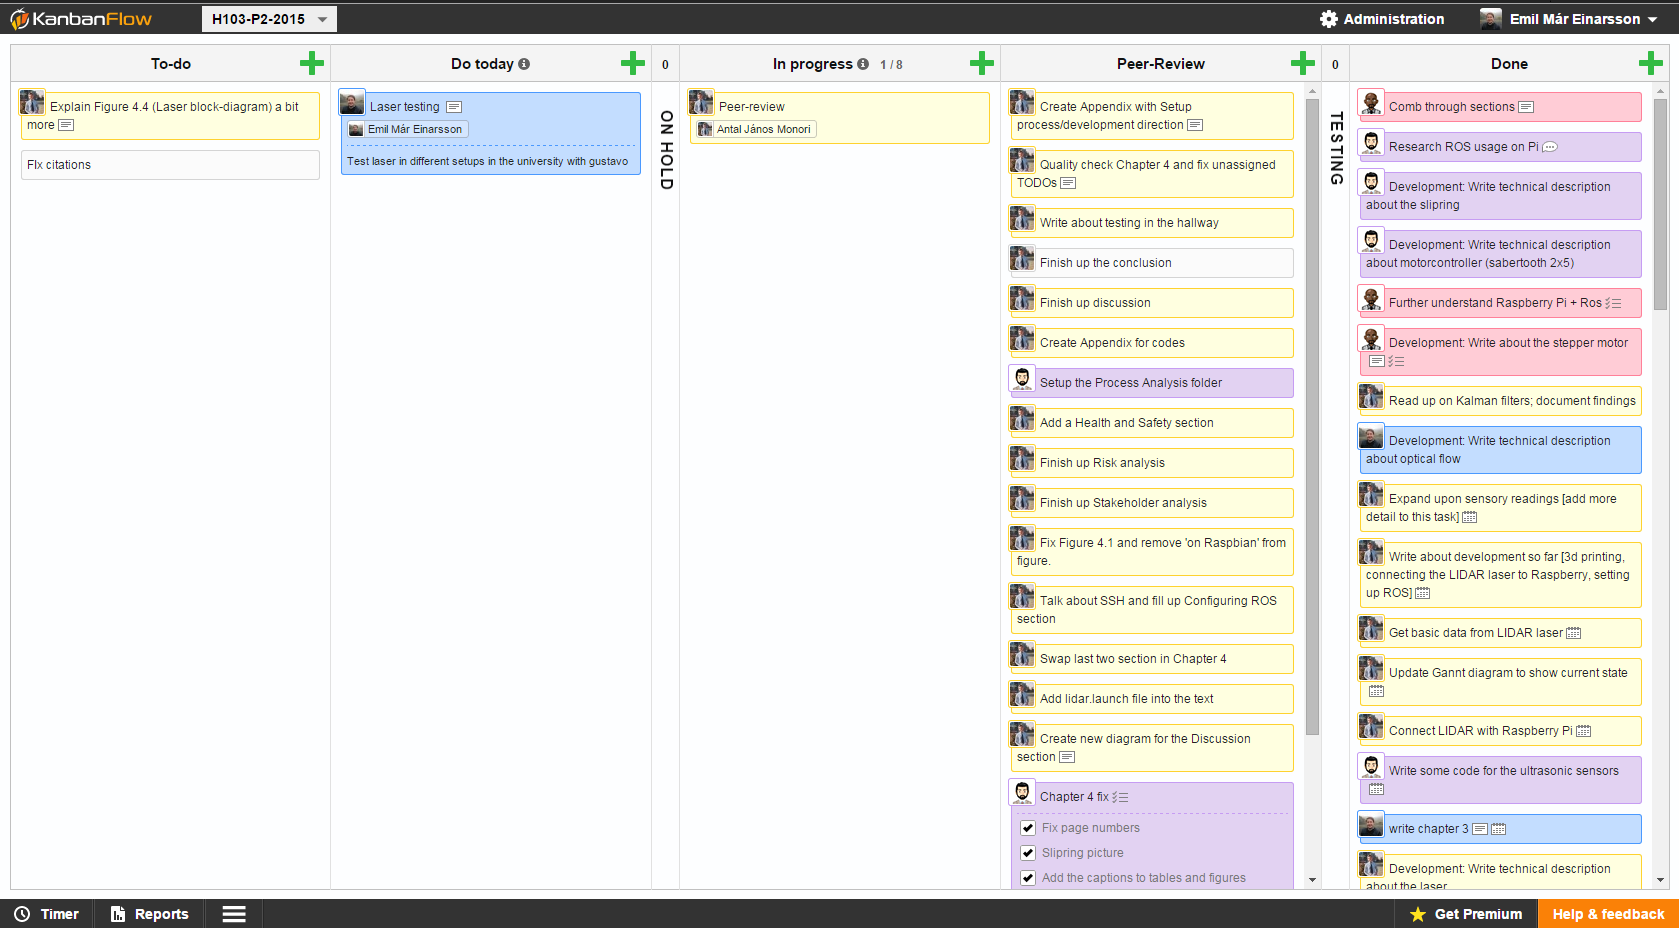
\includegraphics[scale=.35]{images/kanban.png}
	\caption{Our kanban board}
\end{figure}

In the first half of the project, classes had a big effect on how we scheduled meetings and set deadlines for both the big milestones and the smaller tasks. We avoided setting deadlines right after long school days. Because our scope was very large, we often used time allocated to exercises to work on our project instead.

At the end of the project, we weren't satisfied with the state of our prototypes. Because of this, although officially we ended development, we kept trying to tweak the prototype in little ways.

\clearpage
\section{Discussion and Conclusion}

In terms of time and resource management, our biggest downfall was our optimistic time-frame. We did not take into consideration the amount of time needed to learn the tools we used. Our scope was also too large, in the sense that we did not consider that we would need to spend so much time fixing these errors.

Despite our scope being too big, and us running into many more issues than we expected, we were still able to adjust our milestone deadlines, and scope, so that we could finish development with enough time for us to finish the rest of the report. Coming up with a second Gantt-diagram was crucial, since if we had not done it, it would have been much harder for us to tell what we should adjust our scope to.

Another big issue was that we waited too long to order parts, which meant that for around a third of our development, we had nothing to develop. Had we gotten the parts earlier, we might have realised that our scope was too big, and adjust it accordingly.
